\documentclass[11pt,compress,t,notes=noshow, xcolor=table]{beamer}
\usepackage[]{graphicx}\usepackage[]{color}
% maxwidth is the original width if it is less than linewidth
% otherwise use linewidth (to make sure the graphics do not exceed the margin)
\makeatletter
\def\maxwidth{ %
  \ifdim\Gin@nat@width>\linewidth
    \linewidth
  \else
    \Gin@nat@width
  \fi
}
\makeatother

\newcommand{\citebutton}[2]{%
\beamergotobutton{\href{#2}{#1}}%
}

\newcommand{\blu}[1]{\textcolor{blue}{#1}}
\newcommand{\org}[1]{\textcolor{orange}{#1}}
\newcommand{\ques}{\textbf{\textcolor{red}{Question:  }}}
\newcommand{\questionssofar}{\begin{frame}\frametitle{Any questions?}\end{frame}}

\newcommand\warning{%
 \makebox[1.4em][c]{%
 \makebox[0pt][c]{\raisebox{.1em}{\scriptsize!}}%
 \makebox[0pt][c]{\color{red}\normalsize$\bigtriangleup$}}}%

\definecolor{fgcolor}{rgb}{0.345, 0.345, 0.345}
\newcommand{\hlnum}[1]{\textcolor[rgb]{0.686,0.059,0.569}{#1}}%
\newcommand{\hlstr}[1]{\textcolor[rgb]{0.192,0.494,0.8}{#1}}%
\newcommand{\hlcom}[1]{\textcolor[rgb]{0.678,0.584,0.686}{\textit{#1}}}%
\newcommand{\hlopt}[1]{\textcolor[rgb]{0,0,0}{#1}}%
\newcommand{\hlstd}[1]{\textcolor[rgb]{0.345,0.345,0.345}{#1}}%
\newcommand{\hlkwa}[1]{\textcolor[rgb]{0.161,0.373,0.58}{\textbf{#1}}}%
\newcommand{\hlkwb}[1]{\textcolor[rgb]{0.69,0.353,0.396}{#1}}%
\newcommand{\hlkwc}[1]{\textcolor[rgb]{0.333,0.667,0.333}{#1}}%
\newcommand{\hlkwd}[1]{\textcolor[rgb]{0.737,0.353,0.396}{\textbf{#1}}}%
\let\hlipl\hlkwb

\usepackage{framed}
\makeatletter
\newenvironment{kframe}{%
 \def\at@end@of@kframe{}%
 \ifinner\ifhmode%
  \def\at@end@of@kframe{\end{minipage}}%
  \begin{minipage}{\columnwidth}%
 \fi\fi%
 \def\FrameCommand##1{\hskip\@totalleftmargin \hskip-\fboxsep
 \colorbox{shadecolor}{##1}\hskip-\fboxsep
     % There is no \\@totalrightmargin, so:
     \hskip-\linewidth \hskip-\@totalleftmargin \hskip\columnwidth}%
 \MakeFramed {\advance\hsize-\width
   \@totalleftmargin\z@ \linewidth\hsize
   \@setminipage}}%
 {\par\unskip\endMakeFramed%
 \at@end@of@kframe}
\makeatother

\definecolor{shadecolor}{rgb}{.97, .97, .97}
\definecolor{messagecolor}{rgb}{0, 0, 0}
\definecolor{warningcolor}{rgb}{1, 0, 1}
\definecolor{errorcolor}{rgb}{1, 0, 0}
\newenvironment{knitrout}{}{} % an empty environment to be redefined in TeX

\usepackage{alltt}
\newcommand{\SweaveOpts}[1]{}  % do not interfere with LaTeX
\newcommand{\SweaveInput}[1]{} % because they are not real TeX commands
\newcommand{\Sexpr}[1]{}       % will only be parsed by R
\newcommand{\xmark}{\ding{55}}%


\usepackage[english]{babel}
\usepackage[utf8]{inputenc}

\usepackage{dsfont}
\usepackage{verbatim}
\usepackage{amsmath}
\usepackage{amsfonts}
\usepackage{amssymb}
\usepackage{bm}
\usepackage{csquotes}
\usepackage{multirow}
\usepackage{longtable}
\usepackage{booktabs}
\usepackage{enumerate}
\usepackage[absolute,overlay]{textpos}
\usepackage{psfrag}
\usepackage{algorithm}
\usepackage{algpseudocode}
\usepackage{eqnarray}
\usepackage{arydshln}
\usepackage{tabularx}
\usepackage{placeins}
\usepackage{tikz}
\usepackage{setspace}
\usepackage{colortbl}
\usepackage{mathtools}
\usepackage{wrapfig}
\usepackage{bm}
\usepackage{amsmath}
\usepackage{pifont}

\usetikzlibrary{shapes.multipart,shapes,arrows,automata,positioning,calc,chains,trees, shadows}
\tikzset{
  %Define standard arrow tip
  >=stealth',
  %Define style for boxes
  punkt/.style={
    rectangle,
    rounded corners,
    draw=black, very thick,
    text width=6.5em,
    minimum height=2em,
    text centered},
  % Define arrow style
  pil/.style={
    ->,
    thick,
    shorten <=2pt,
    shorten >=2pt,}
}

\tikzstyle{vec}=[draw, rectangle, fill = white, minimum width=5mm, minimum height=1cm, inner sep = 2pt]

\usepackage{subfig}

% Defines macros and environments
\usepackage{../../style/lmu-lecture}


\let\code=\texttt
\let\proglang=\textsf

\setkeys{Gin}{width=0.9\textwidth}

\setbeamertemplate{frametitle}{\expandafter\uppercase\expandafter\insertframetitle}

\usepackage{bbm}
% basic latex stuff
\newcommand{\pkg}[1]{{\fontseries{b}\selectfont #1}} %fontstyle for R packages
\newcommand{\lz}{\vspace{0.5cm}} %vertical space
\newcommand{\dlz}{\vspace{1cm}} %double vertical space
\newcommand{\oneliner}[1] % Oneliner for important statements
{\begin{block}{}\begin{center}\begin{Large}#1\end{Large}\end{center}\end{block}}


%new environments
\newenvironment{vbframe}  %frame with breaks and verbatim
{
 \begin{frame}[containsverbatim,allowframebreaks]
}
{
\end{frame}
}

\newenvironment{vframe}  %frame with verbatim without breaks (to avoid numbering one slided frames)
{
 \begin{frame}[containsverbatim]
}
{
\end{frame}
}

\newenvironment{blocki}[1]   % itemize block
{
 \begin{block}{#1}\begin{itemize}
}
{
\end{itemize}\end{block}
}

\newenvironment{fragileframe}[2]{  %fragile frame with framebreaks
\begin{frame}[allowframebreaks, fragile, environment = fragileframe]
\frametitle{#1}
#2}
{\end{frame}}


\newcommand{\myframe}[2]{  %short for frame with framebreaks
\begin{frame}[allowframebreaks]
\frametitle{#1}
#2
\end{frame}}

\newcommand{\remark}[1]{
  \textbf{Remark:} #1
}


\newenvironment{deleteframe}
{
\begingroup
\usebackgroundtemplate{
\includegraphics[width=\paperwidth,height=\paperheight]{../style/color/red.png}}
 \begin{frame}
}
{
\end{frame}
\endgroup
}
\newenvironment{simplifyframe}
{
\begingroup
\usebackgroundtemplate{
\includegraphics[width=\paperwidth,height=\paperheight]{../style/color/yellow.png}}
 \begin{frame}
}
{
\end{frame}
\endgroup
}\newenvironment{draftframe}
{
\begingroup
\usebackgroundtemplate{
\includegraphics[width=\paperwidth,height=\paperheight]{../style/color/green.jpg}}
 \begin{frame}
}
{
\end{frame}
\endgroup
}
% https://tex.stackexchange.com/a/261480: textcolor that works in mathmode
\makeatletter
\renewcommand*{\@textcolor}[3]{%
  \protect\leavevmode
  \begingroup
    \color#1{#2}#3%
  \endgroup
}
\makeatother





\input{../../latex-math/basic-math.tex}
\input{../../latex-math/basic-ml.tex}

\newcommand{\titlefigure}{figure/sesamestreet.jpeg}
\newcommand{\learninggoals}{
\item Understand the improvements over BERT
\item Permutation language modeling
\item }

\title{Using the Transformer}
% \author{}
\institute{\href{https://slds-lmu.github.io/lecture_dl4nlp/}{slds-lmu.github.io/lecture\_dl4nlp}}
\date{}

\begin{document}
\lecturechapter{XLNet (Yang et al., 2019)}
\lecture{Deep Learning for NLP}

% ------------------------------------------------------------------------------

\begin{frame}{XLNet \href{https://papers.nips.cc/paper/8812-xlnet-generalized-autoregressive-pretraining-for-language-understanding.pdf}{\beamergotobutton{Yang et al., 2019}}}

	\textbf{Autoregressive (AR) language modeling vs. Autoencoding (AE)}
	
	\begin{itemize}
		\item \textit{AR:} Factorizes likelihood to $p(\mathbf{x}) = \prod_{t=1}^{T} p(x_t | \mathbf{x}{< t})$
		\item Only uni-directional (backward factorization instead would also be possible)
		\item \textit{AE:} Objective to reconstruct masked tokens $\bar{\mathbf{x}}$ from corrupted sequence $\hat{\mathbf{x}}$:
					$p(\bar{\mathbf{x}}|\hat{\mathbf{x}}) = \prod_{t=1}^{T} m_t \cdot p(x_t | \hat{\mathbf{x}})$, $m_t$ as masking indicator
	\end{itemize}

	\vspace{.3cm}
	
	\textbf{Drawbacks / Advantages}
	
	\begin{itemize}
		\item No corruption of input sequences when using AR approach
		\item AE approach induces independence assumption between corrupted tokens
		\item AR approach only conditions on left side context\\$\Rightarrow$ No bidirectionality
	\end{itemize}
\end{frame}

% ------------------------------------------------------------------------------

\begin{frame}{Alternative objective funktion}

	\textbf{Permutation language modeling (PLM)}
	
	\begin{itemize}
		\item Solves the pretrain-finetune discrepancy
		\item Allows for bidirectionality while keeping AR objective
		\item Consists of two "\textit{streams}" of the Attention mechanism
				\begin{itemize}
					\item Content-stream attention
					\item Query-stream attention
				\end{itemize}
	\end{itemize}

	\vspace{.3cm}
	
	\textbf{Manipulating the factorization order}
	
	\begin{itemize}
		\item Consider permutations $\mathbf{z}$ of the index sequence $[1,2, \hdots, T]$\\
					$\rightarrow$ Used to permute the factorization order, \textit{not} the sequence order.
		\item Original sequence order is retained by using positional encodings
		\item PLM objective (with $\mathcal{Z}_T$ as set of all possible permutations):
					$$\max_{\theta} \quad \mathds{E}_{\mathbf{z}\sim\mathcal{Z}_T} \left[ \sum_{t=1}^{T} \log p_\theta (x_{z_t} | \mathbf{x}_{\mathbf{z}_{< t}}) \right]$$
	\end{itemize}
\end{frame}

% ------------------------------------------------------------------------------

\begin{frame}{Content- vs. Query-stream}

	\textbf{Content-stream}
	
	\begin{itemize}
		\item "Normal" Self-Attention (despite with special attention masks)\\
					$\rightarrow$ Attentions masks depend on the factorization order
		\item Info about the position in the sequence is lost, see \href{https://arxiv.org/pdf/1906.08237.pdf}{\beamergotobutton{Example in A.1}}
		\item Sets of queries ($Q$), keys ($K$) and values ($V$) from content stream*
		\item Yields a \textit{content embedding} denoted as $h_{\theta}(\mathbf{x}_{\mathbf{z}_{\leq t}})$
	\end{itemize}

	\vspace{.3cm}
	
	\textbf{Query-stream}
	
	\begin{itemize}
		\item Access to context through content-stream, but no access to the content of the current position (only location information)
		\item $Q$ from the query stream, $K$ and $V$ from the content stream*
		\item Yields a \textit{query embedding} denoted as $g_{\theta}(\mathbf{x}_{\mathbf{z}_{< t}}, z_t)$
	\end{itemize}

	\vspace{.3cm}
	
	{\footnotesize *For a nice visual disentanglement, see \href{https://arxiv.org/pdf/1906.08237.pdf}{\beamergotobutton{Figures in A.7}}}
\end{frame}

% ------------------------------------------------------------------------------

\begin{frame}{XLNet -- Graphical representation}
	\begin{figure}
		\centering
		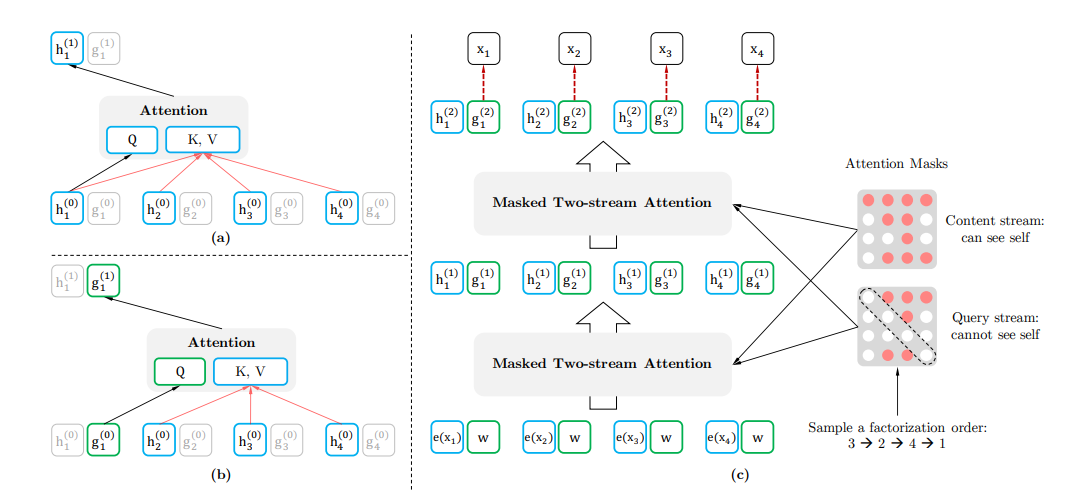
\includegraphics[width = 12cm]{figure/xlnet}\\ 
		{\tiny (a) content-stream; (b) query-stream; (c) whole model\\\footnotesize Source: \href{https://papers.nips.cc/paper/8812-xlnet-generalized-autoregressive-pretraining-for-language-understanding.pdf}{Yang et al. (2019)}}
	\end{figure}
\end{frame}

% ------------------------------------------------------------------------------

\begin{frame}{XLNet -- Model Input}

\textbf{Generation of samples:}

\begin{itemize}
\item Randomly sample two sentences and use concatenation* as input
			{\footnotesize
\begin{center}
\begin{tabular}{|cccccccc|}
\hline
\cellcolor{blue!15}\texttt{[CLS]} & The & fox & is & quick & . & \cellcolor{blue!15}\texttt{[SEP]} &\\\hline\hline It & jumps & over & the & lazy & dog & . & \cellcolor{blue!15}\texttt{[SEP]} \\
\hline
\end{tabular}\\\mbox{}
\end{center}}
{\scriptsize *Nevertheless: XLNet does \textit{not} use the NSP objective }
\end{itemize}

\textbf{Additional encodings:}

\begin{itemize}
\item \textit{Relative} segment encodings:
	\begin{itemize}
		\item BERT adds absolute segment embeddings ($E_A$ \& $E_B$)
		\item XLNet uses relative encodings ($\vec{s}_+$ \& $\vec{s}_-$)
	\end{itemize}
\item \textit{Relative} Positional encodings:
	\begin{itemize}
		\item BERT encodes information about the absolute position ($E_0, E_1, E_2, \hdots$)
		\item XLNet uses relative encodings ($R_{i - j}$)
	\end{itemize}
\end{itemize}
\end{frame}

% ------------------------------------------------------------------------------

\begin{frame}{XLNet -- Special remarks}
	
	\begin{itemize}
		\item \textbf{Partial Prediction:} Only predict the last tokens in a factoriztion order (reduces optimization difficulty)
					{\small $$\max_{\theta} \quad \mathds{E}_{\mathbf{z}\sim\mathcal{Z}_T} \left[ \sum_{t=c+1}^{|\mathbf{z}|} \log p_\theta (x_{z_t} | \mathbf{x}_{\mathbf{z}_{< t}}) \right],\quad \mbox{with $c$ as cutting point}$$}
		\item \textbf{Segment recurrence mechanism:} Allow for learning extended contexts in Transformer-based architectures, see \href{https://arxiv.org/pdf/1901.02860.pdf}{\beamergotobutton{Dai et al. (2019)}}
		\item \textbf{No independence assumption:}
	\begin{figure}
		\centering
		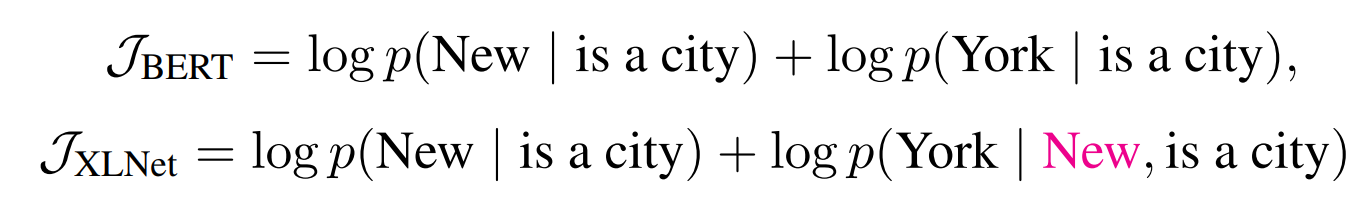
\includegraphics[width = 9cm]{figure/xlnet-objective}\\ 
		{\tiny Prediction of [New, York] given the factorization order [is, a, city, New, York]\\\footnotesize Source: \href{https://papers.nips.cc/paper/8812-xlnet-generalized-autoregressive-pretraining-for-language-understanding.pdf} \it Yang et al. (2019)}
	\end{figure}
	\end{itemize}
\end{frame}

% ------------------------------------------------------------------------------

\begin{frame}{XLNet -- SOTA performance}
\small
	\textbf{Performance differences to BERT:}

	\begin{figure}
		\centering
		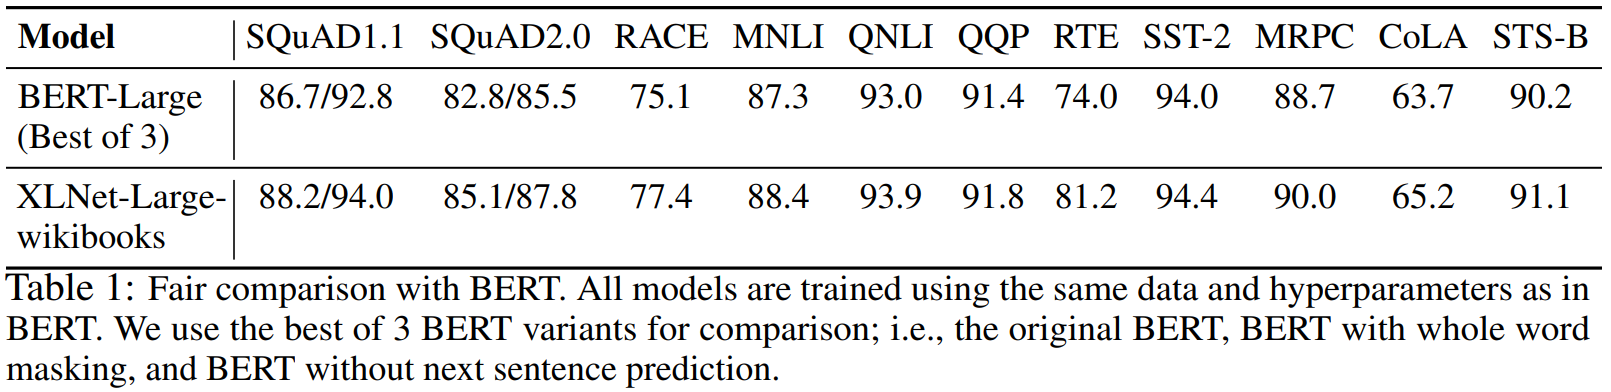
\includegraphics[width = 9cm]{figure/xlnet-vs-bert.png}\\ 
		\footnotesize{Source:} \href{https://papers.nips.cc/paper/8812-xlnet-generalized-autoregressive-pretraining-for-language-understanding.pdf}{\footnotesize Yang et al. (2019)}
	\end{figure}

	\textbf{SOTA performance:}

	\begin{figure}
		\centering
		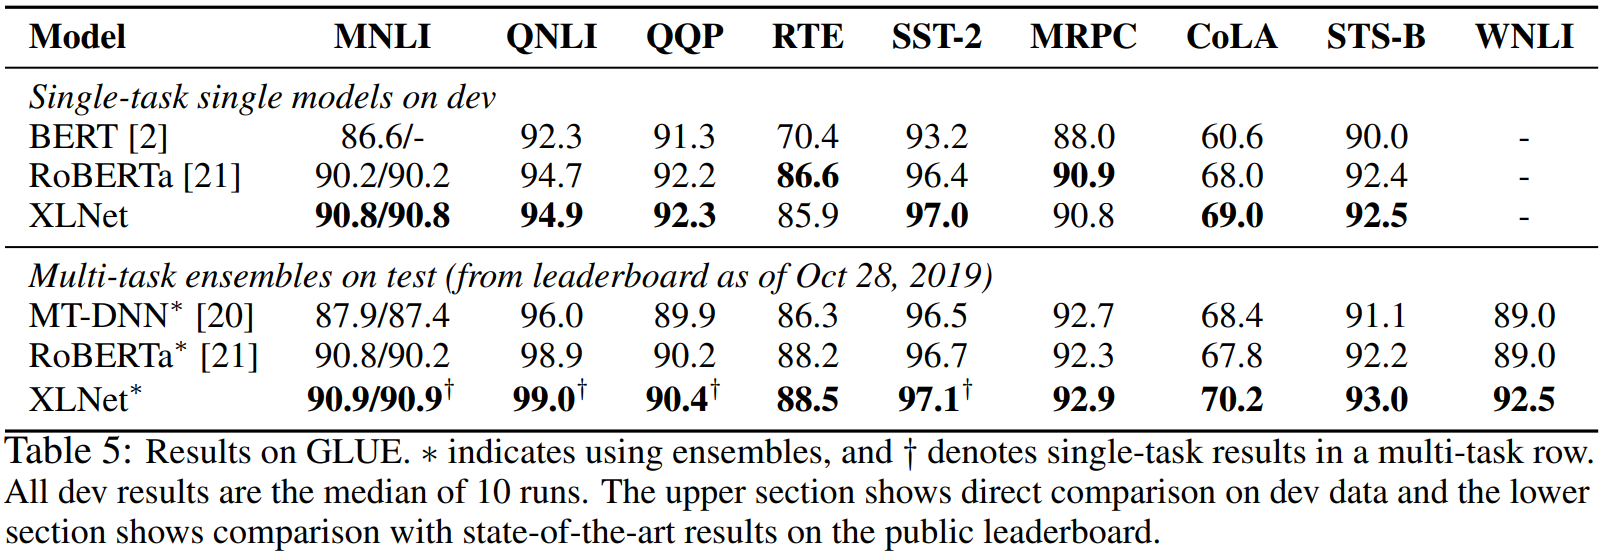
\includegraphics[width = 9cm]{figure/xlnet-sota.png}\\ 
		\footnotesize{Source:} \href{https://papers.nips.cc/paper/8812-xlnet-generalized-autoregressive-pretraining-for-language-understanding.pdf}{\footnotesize Yang et al. (2019)}
	\end{figure}
\end{frame}

% ------------------------------------------------------------------------------

\endlecture
\end{document}
